\chapter{Regionally Containing Epidemics \RNum{1}: Modelling Ash dieback}


% Fifth: Narrow in on what this paper aims to do and what specifically is novel
The spatial structure of plant-hosts is an important factor when considering how to manage %
an epidemic \cite{spatial-control-optimisation, control-heterogeneous-landscapes}. %
In this work, we model how host-heterogeneity, under the influence of an %
\textcolor{red}{arbitrary pathogen}, can give rise to natural pinch-points and fault-lines %
in the spatial population. %
In principle, this could be exploited with targeted tree felling in order to efficiently %
fragment the host population with minimised effort. %
If the pathogen is laying inside a disconnected fragment of the host population, %
it will remain localised and the epidemic will be prevented from spreading large distances. %
Similar concepts have been outlined for crop and livestock diseases \cite{PAPAIX201435, GILIOLI20131, Gilligan-disease-management}. %
However, to our knowledge, this has not been generalised to tree population distributions. %
Additionally, no modelling have been attempted to optimise for epidemic control, based only %
on the structure of a large-scale, spatial distribution of hosts and incorporating topography.\\

Section \textcolor{red}{RESULTS} details the ensemble averaged results of the sub-grid model %
and explains further how to generate $R_0$-maps for the Ash population under the influence of %
a given pathogen. %
An image processing technique is then applied to the $R_0$-map in order to identify high-risk %
clusters of Ash. Considering the structure of high-risk clusters, we illustrate how targeted %
tree felling may disconnect large areas of the population into fragments and show how this %
can be used to contain an epidemic. Lastly, the efficiency of fragmentation is explored by %
assessing the number of trees, saved in relation to the number felled. We end in Section %
\textcolor{red}{DISCUSSION} with a discussion on the applicability, limitations and potential %
extensions of our developed model. %

There are many pathways a pathogen can use to spread through a landscape. %
These include long-range dispersal, mediated through either human-trade networks %
\cite{hulme2009trade, banks2015role, chapman2017global} or dispersal in the upper atmosphere %
\cite{westbrook1999atmospheric, isard2005principles}. %
We are interested in dispersal at the local, landscape level, whereby dispersal may occur %
naturally through the passive means of wind, soil and or insects. %

 


\subsection{Constructing a simplified model of ash dieback model}

\begin{table}[h]
\centering
\begin{tabular}{l l l}
\hline
\textbf{Model parameter} & \textbf{Description} & \textbf{Typical value(s)}\\
\hline
$\rho$  & Tree density & $0.00 - 0.10$ \\ 
$\beta$ & Infectivity & $0.00010 - 0.00100\ \mathrm{day}^{-1}$ \\
$\ell_{ga}$ & Pathogen dispersal distance & $196\mathrm{m}$ \\
$T$ & Sporulation peak & $120$ days from June - September \\
$t$ & Time-step & $[0, T]$ days\\
$R_0$ & Mean reproduction number & $0-20$ \\
$\mathcal{L}$ & Lattice dimension & $1000\times1000$ \\
$\mathcal{A}$ & Domain area & $5\mathrm{km}\times5\mathrm{km}$ \\
$\gamma$ & Lattice constant & $5\mathrm{m}$ \\
\hline
\end{tabular}
\caption{Model parameters}
\end{table}


We begin with a homogeneous distribution of trees, informed by a density parameter $\rho$, inside a square domain of size $\mathcal{L}$. Each lattice-point represents a $5m\times5m$ patch of land that is occupied by a an ash tree, with probability $\rho$, or empty with probability $(1-\rho)$. The state of a tree can be in one of four compartments and trees transition between $S\rightarrow E \rightarrow I \rightarrow R$, without the possibility of recover. We consider two dispersal kernels, a thin-tailed Gaussian and a fat-tailed power-lower.

Given two trees, one susceptible ($S_x$) and one infected ($I_{x^\prime}$), separated by a distance $r$, an expected transition rate for $S_x \rightarrow E_x$ can be determined from the dispersal kernel multiplied by an infectivity rate $\beta$. For Gaussian and power-law this assumes the form:

\begin{equation}
    Pr(S_{x} \rightarrow E_{x} ;\ I_{x^{\prime}} ) = \beta  \phi(T) \exp\Big[\frac{-r^2}{2\ell^2}\Big] 
\end{equation}
\begin{equation}
    Pr(S_{x} \rightarrow E_{x} ;\ I_{x^{\prime}} ) = \beta \phi(T) (1 - r/\ell)^{-r}
\end{equation}

A simple time-dependant function $\phi(T)$ takes the value of $1$ between the summer months of June - September, and $0$ otherwise thus reflecting the sporulation peak of \textit{Hymenoscyphus fraxineus}. During these summer months, wind-borne dispersal occurs when fruiting bodies produce large numbers of ascospores. 

We make an assumption that trees transitioning from $E\rightarrow E; I_{n}$
We make an assumption that trees transitioning from $S\rightarrow E$ on account of infected tree $I_{n}$, will only become infectious to neighbouring trees during the following sporulation peak, denoted by $S\rightarrow E; I_{n+1}$. This is justified given the strong seasonal component in the life cycle of \textit{Hymenoscyphus fraxineus}\textemdash that is, where infected trees shed plant-material which 
becomes infectious during the following sporulation peak. 

a basic reproduction number $R_0$ is defined for the first life-cycle of the pathogen.
It takes approximately $2-4$ months for an infected ash tree to become symptomatic. However, given that dispersal via the wind-borne mechanism only occurs during the summer months we make the assumption that trees in the exposed category will only become infectious in the next sporulation peak





\begin{figure}
    \centering
    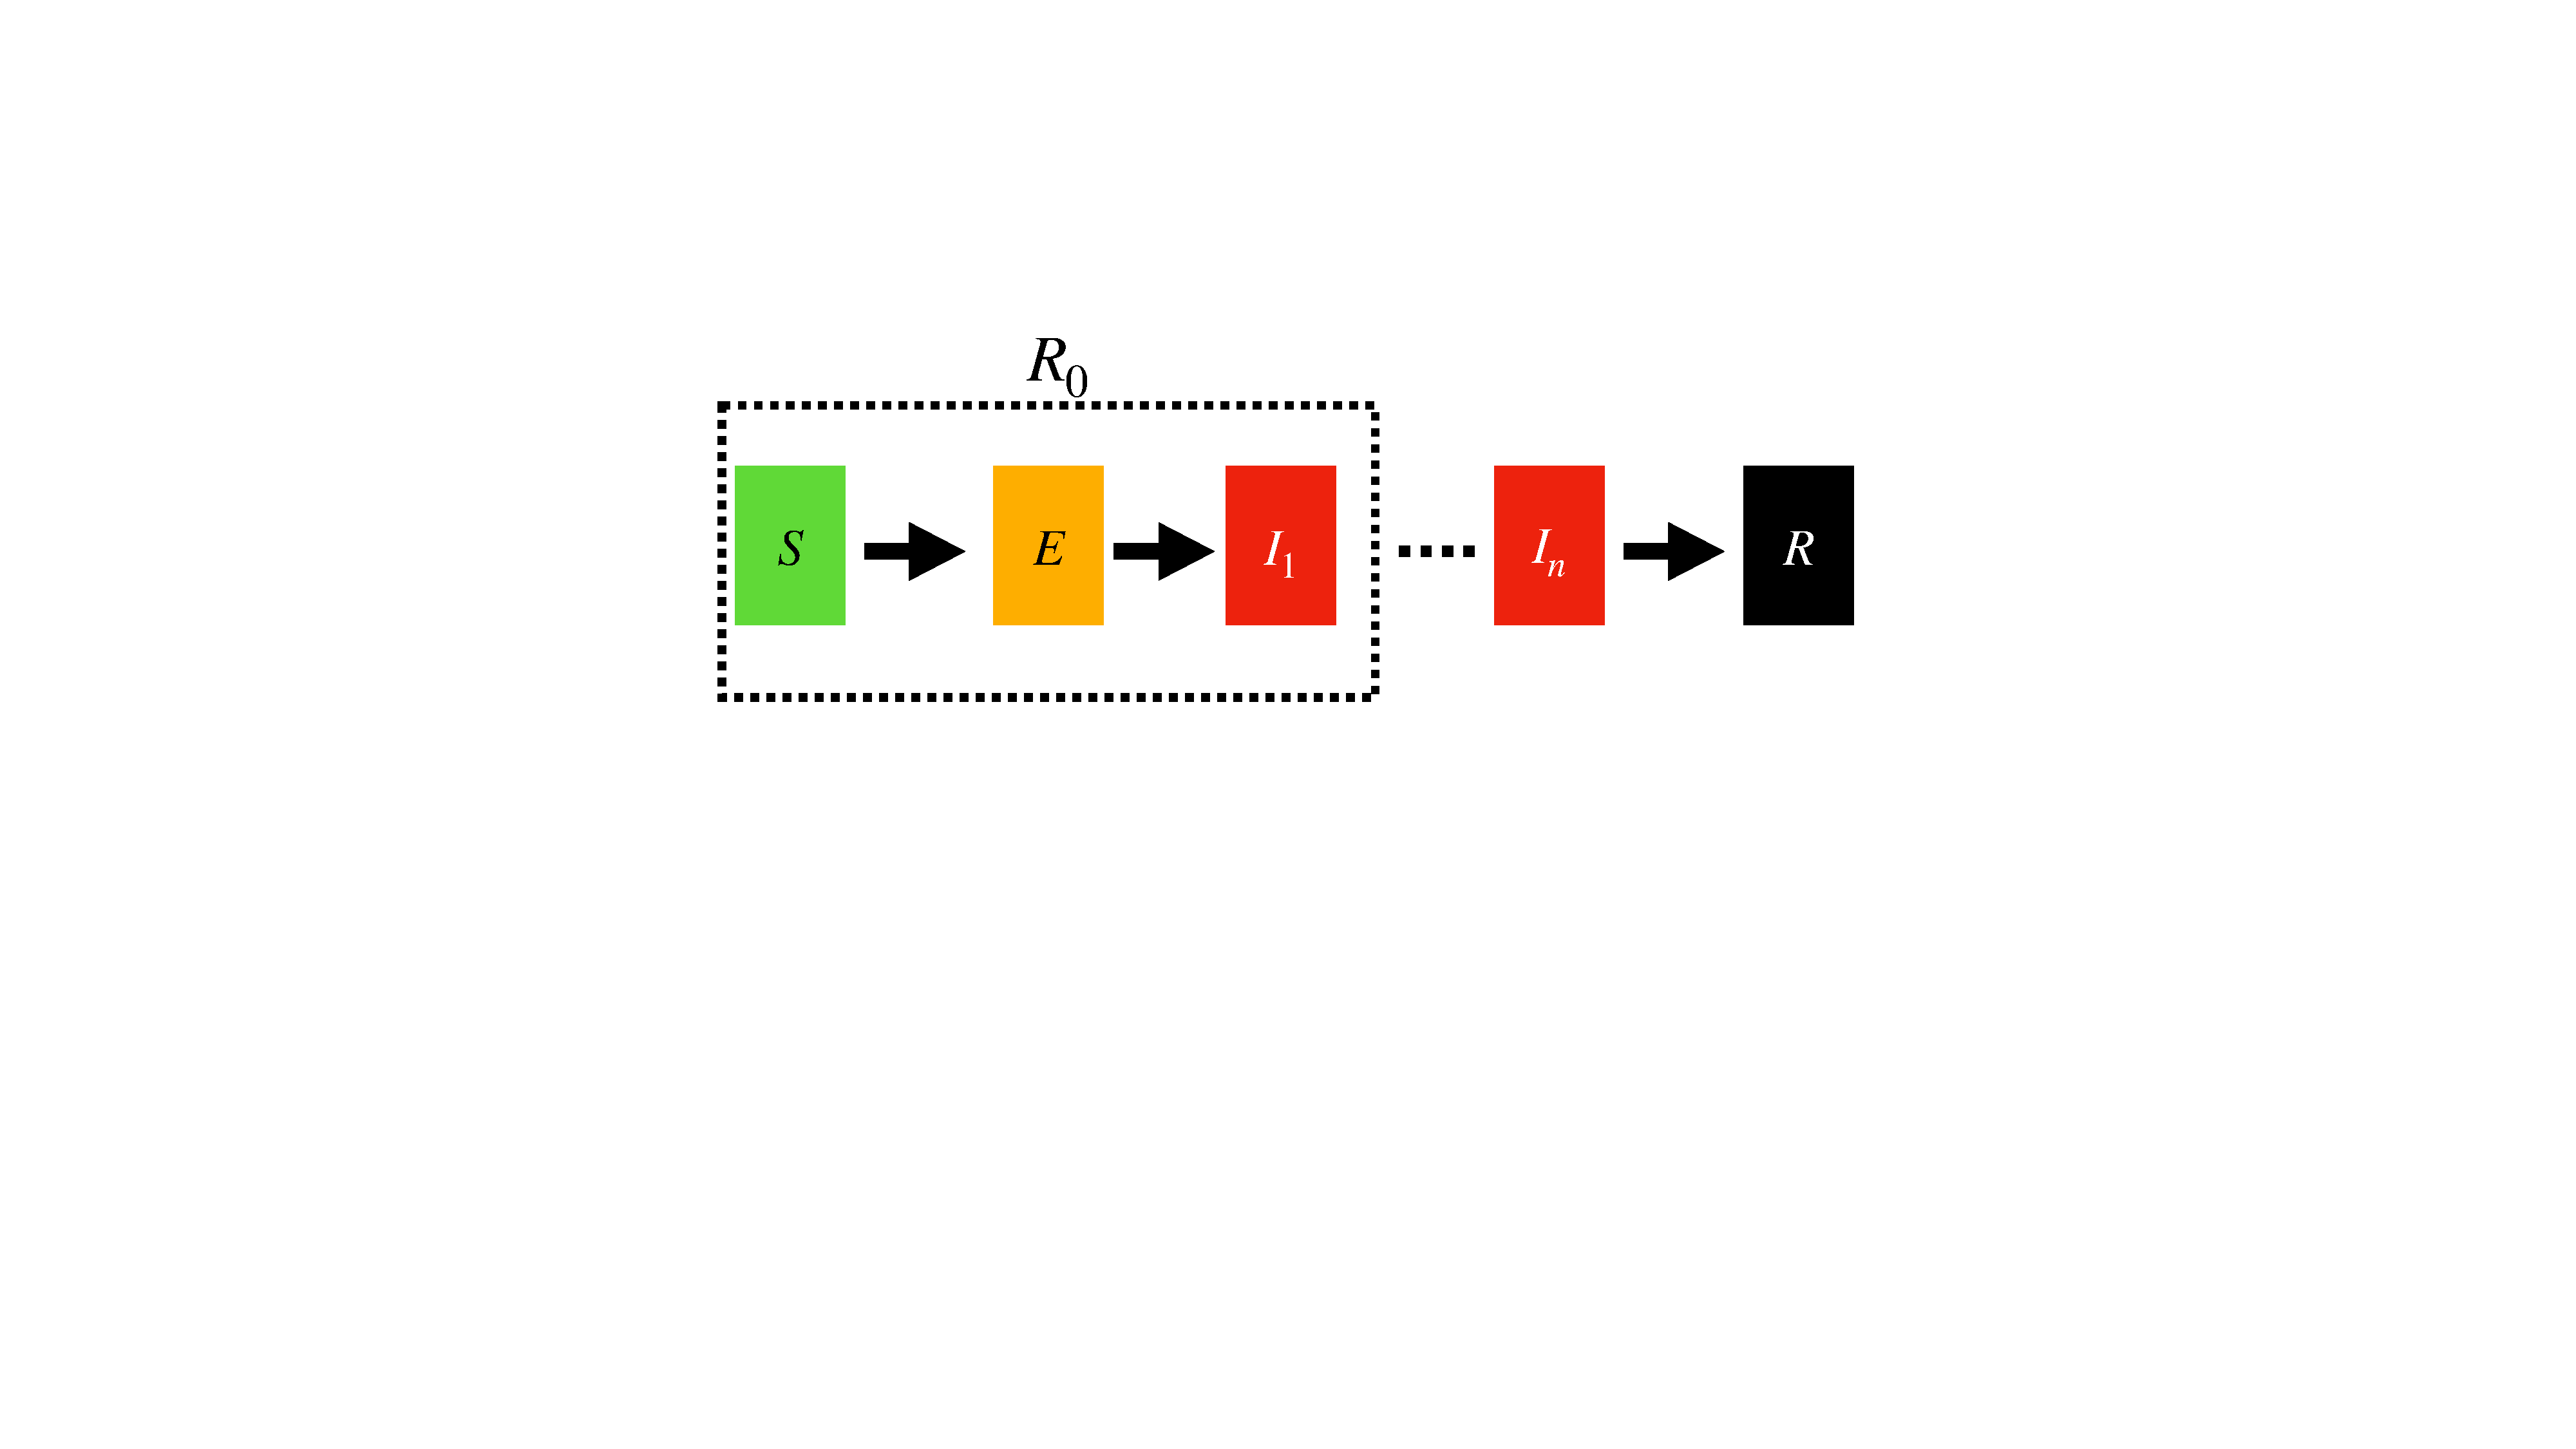
\includegraphics[scale=0.30]{chapter5/figures_/fig4.pdf}
    \caption{The $SEIR$ model of ash dieback.}
    \label{fig:my_label}
\end{figure}

\textcolor{red}{
\begin{itemize}
    \item The majority of fruiting bodies are produced during the late summer months, that is, the sporulation peak. The model will describe the dispersal of these fruiting bodies over these ensuing months from June-August --reference sporulation peak extensively
    \item The model is a spatial SIR where infectious trees transition to the R compartment at the end of the season when trees cease to become infective -- in this case, trees are still alive but assumed to remain in a dormant state until next summer --reference biology and dormancy of ash db
    \item the infectious trees transition to the R compartment at with rate parameter $\gamma = 1/30$ such that at the end of two months the probability of the tree still producing infectious spores is approximately $10\%$ and at the end of three months is $5\%$
\end{itemize}
}


\subsection{Producing $R_0$-maps and informed dispersal}

\begin{figure}
    \centering
    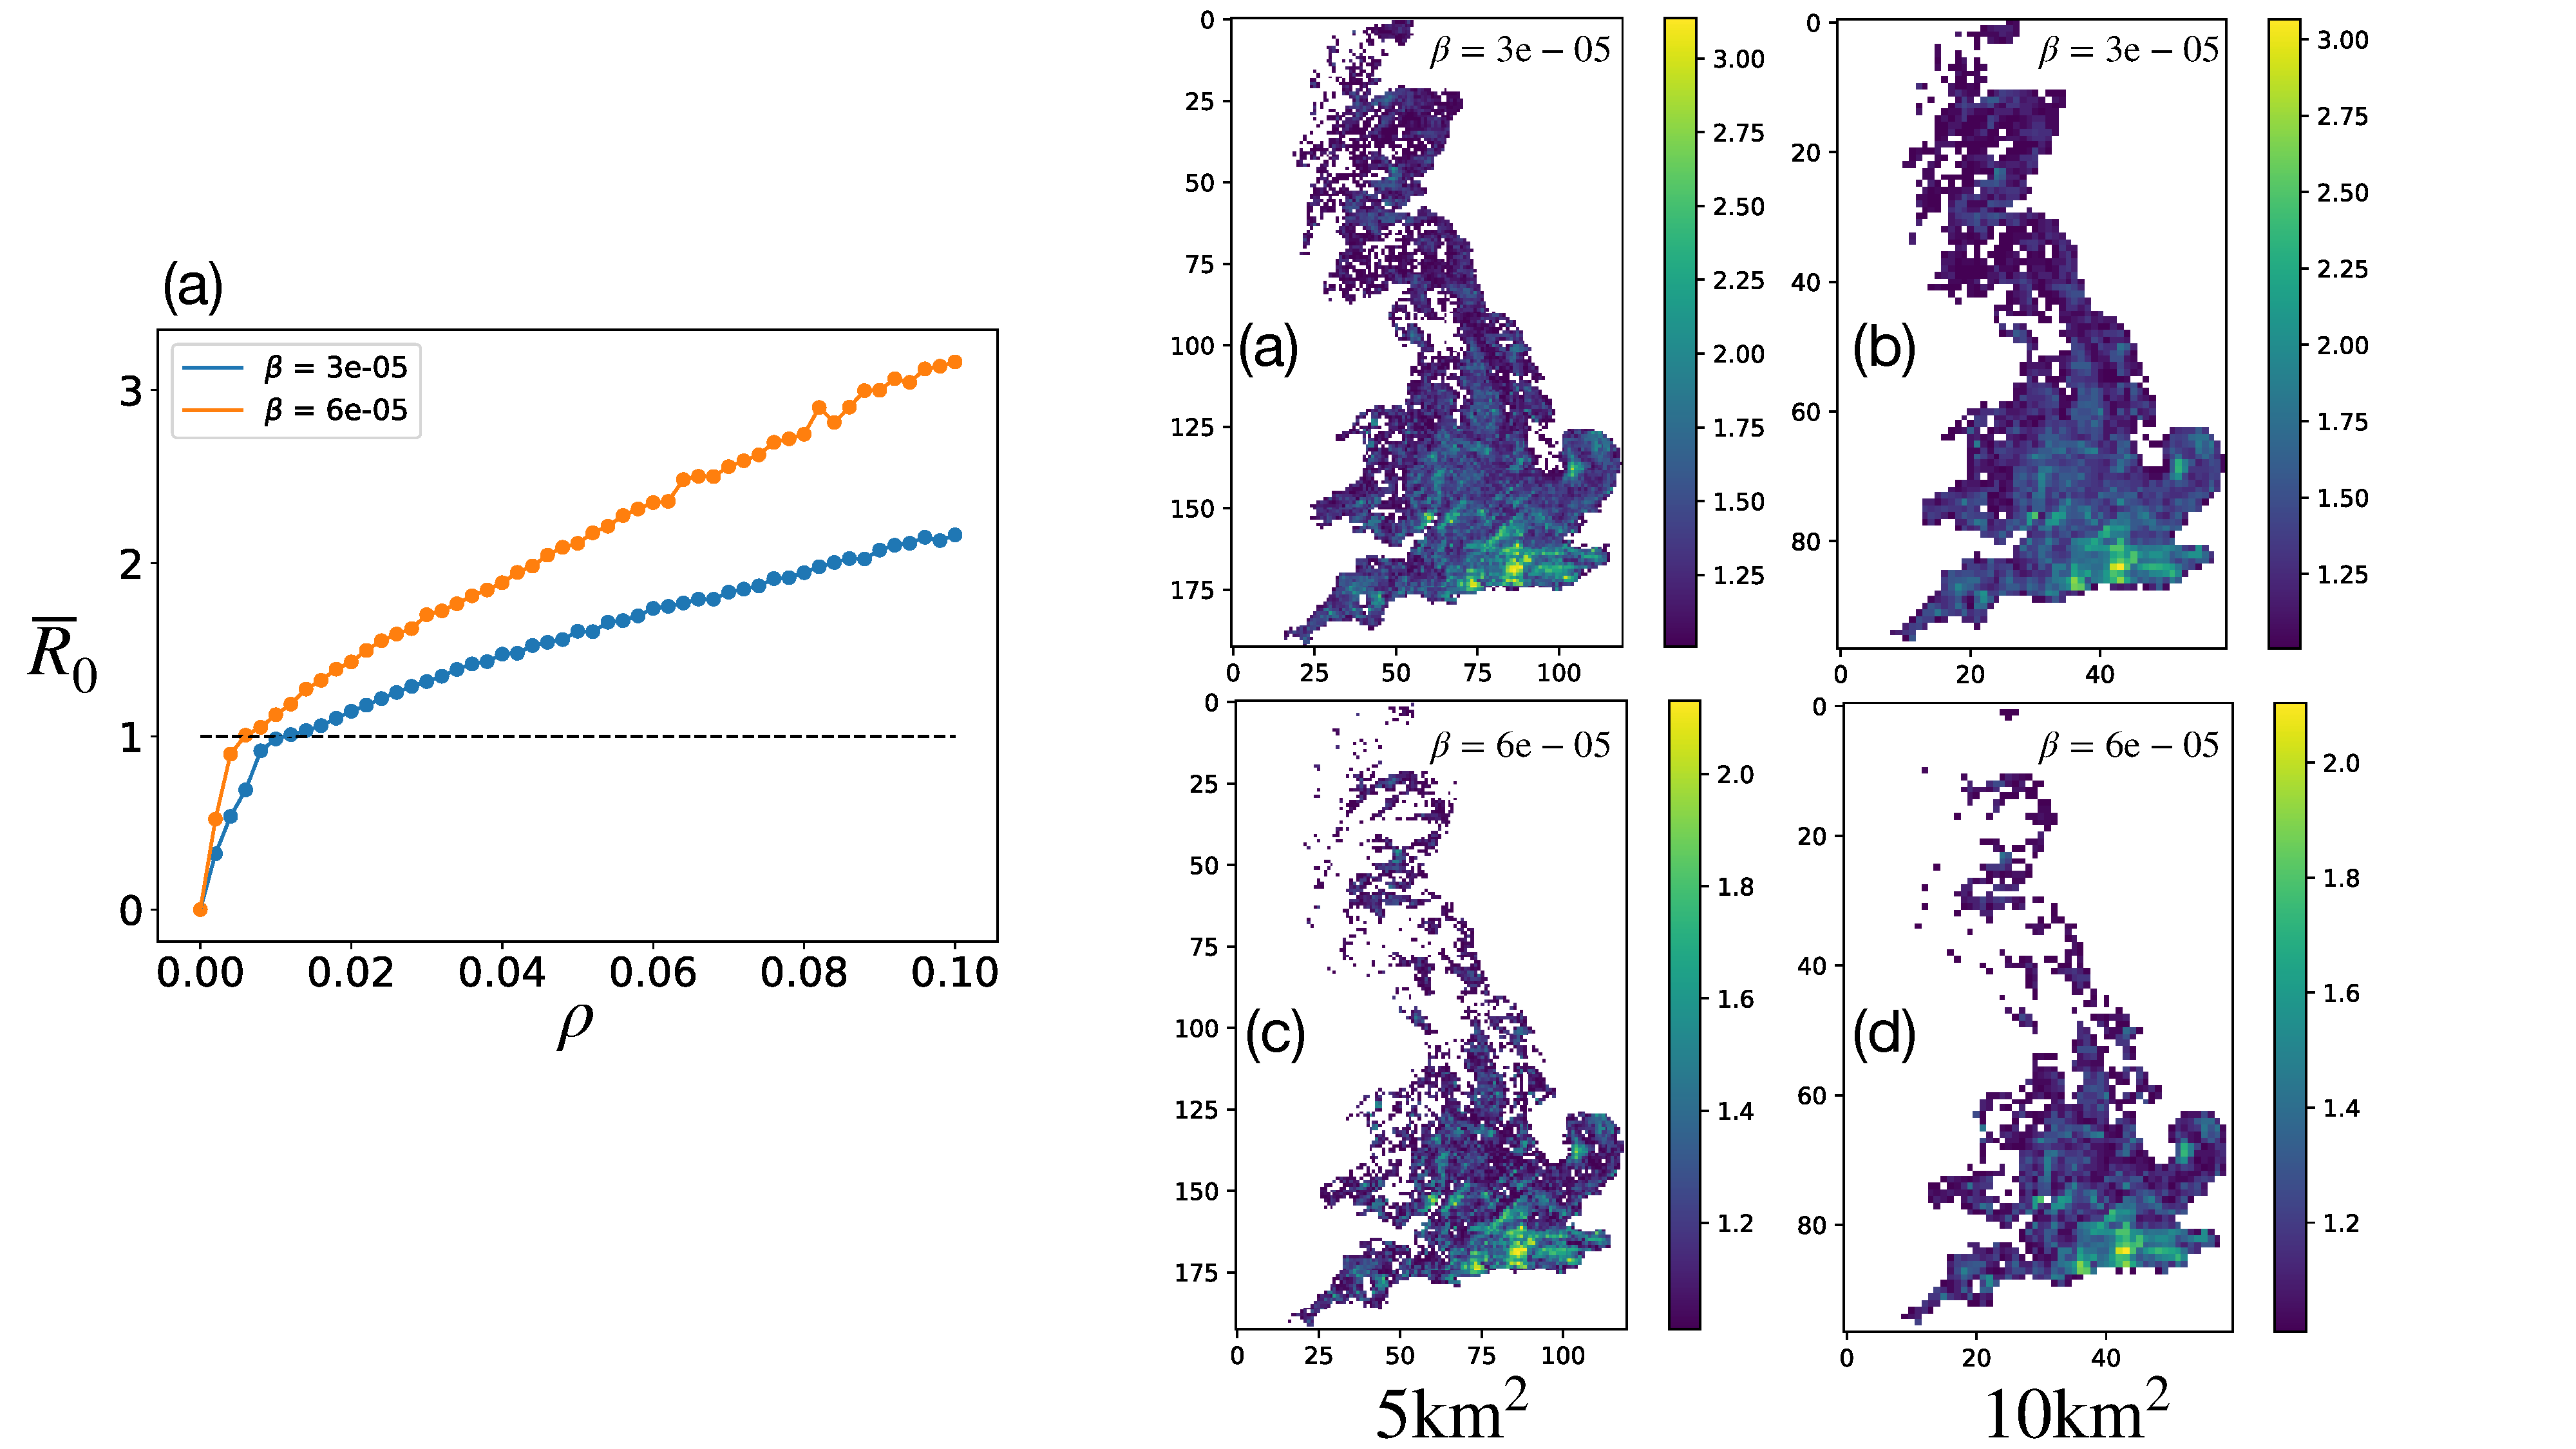
\includegraphics[scale=0.25]{chapter5/figures_/fig3.pdf}
      \caption{(a) Ensemble-averaged $R_0$ between two values of $\beta$, for Gaussian dispersal of $\ell=1.6\mathrm{km}$. (a-b) $R_0$-map for $\beta=3\mathrm{e}-05$, coarse-grained at $5$, $ 10\mathrm{km^2}$. (c-d) $R_0$-map for $\beta=6\mathrm{e}-05$.}
    \label{fig:mapping-R0-onto-density}
\end{figure}

\textcolor{red}{
\begin{itemize}
    \item We compare two kernels, a Gaussian and inverse power-law. The scale dispersal is set using parameter-values inferred by a study conducted in France \cite{grosdidier2018tracking}. In this study, the authors using a trapping-method to infer the mean distance travelled by a fungal-spore from a source of inoculum at various spatial scales. The values ascertained at the local-scale /footnote(governed primarily by airborne dispersal), which is spatial-scale we are interested in, was found to be $0.17\mathrm{km}$ and $1.38\mathrm{km}$ for the Gaussian and inverse power-law kernels respectively.
    That is, a fungal spore will travel a mean distance of $0.17\mathrm{km}$
    \item Discuss mapping $R_0$ to tree density, \ref{fig:mapping-R0-onto-density} 
    \item Discuss the role of domain resolution--loss or gain of spatial structure in $R_0$ map
    \item Discuss how the choice of resolution should be tailored to the spatial resolution of $R_0$-map and how this relates to informed dispersal
\end{itemize}
}

\subsection{The identification of $R_0$-clusters}

\textcolor{red}{
\begin{itemize}
    \item Show the construction of $R_0$ cluster-detection, consider the top $10$ say, for some arbitrary $\beta$ values and the chosen structuring element (either Moore or Von Nuemann, whichever performs the best)
    \item show that as $\beta$ increases clusters become larger, illustrate this with a plot of cluster-size vs $\beta$ (over Gaussian and power-law dispersal)
    \item run a second analysis using the remaining structuring element (either Moore or Von Nuemann, dependent on which element you choose to run the main analysis)
\end{itemize}}


\subsection{Cluster-fragmentation}

\textcolor{red}{
\begin{itemize}
    \item show cluster fragmentation of a few artificially constructed domains with obvious boundaries
    \item Discuss cluster-fragmentation and illustrate how this achieved diagrammatically: 1) for one value of beta/rho/ell, show that clusters grow and connect as $\alpha \rightarrow max(R_0)$. 2) show that at points in $\alpha$-space, cluster-joins occur which are products of the spatial structure 3) describe that the cluster-joins are identified using the largest rise in cluster size, which occurs when two or more clusters connect
    \item show how connector-patches are detected using the binary dilation operator: 1) that cluster-targets are tracked for each step, and if they become connected we know there has been a join 2) you take the binary dilatation of the negated cluster-targets 3) positions which become non-zero and touch the perimeter are candidates for removal etc. 4) that which ever cluster C1, C2 has the lowest number of joins, is targeted for removal. 5) Illustrate how fragmentation-iterations successively target the largest sub-cluster after fragmentation
    \item in the appendix, describe 1) the initial conditions of alpha 2) how cluster joins are handled for multi-joins 3) The binary dilation operator in more detail 4) the packages used in this computation 
\end{itemize}
}

\subsection{Culling payoff; results over $\beta$ }

\textcolor{red}{
\begin{itemize}
    \item Discuss how combinations of fragmentations iterations can be used to workout the optimal containment for a given epicenter
    \item Show the culling payoff over the infectivity space--illustrate this over the space of $\beta$. Hopefully, you will see a $\beta$-regime where the payoff has a maximum
    \item Discuss the high-payoff scenarios, important identification of central-joins and subsequent culling -- illustrate this with map saved, culled and removed patches
    \item Discuss the epidemiological interpretation of $R_0$-maps over $\beta$. That is, when $\beta$ is low, the map shows significant fragmentation. In this scenario, the spread of disease in this model would only be possible with significant long distance dispersal-mechanisms. Here, a conjecture may be made about the human-transport being the most effective pathway to target. Alternatively, when $\beta$ is higher and the map is connected...
\end{itemize}}
\subsection{Informing $\beta$}
\textcolor{red}{
This section is more of a conjecture at this point
\begin{itemize}
    \item From observations around Europe, the disease-front spreads at a typical rate or $50-60 km/yr$
    \item It might therefore be possible to use our $SEIR$-model, with informed parameters, to ascertain a value of $\beta$ which gives this rate of spread. For an order-of-magnitude estimate, we could run this simulation over the mean tree density of the UK.
    \item A number of problems would need to be solved before this could be implemented: 
    \begin{enumerate}
        \item Making/ensuring the model runs in good-time on a large domain $10-20 \mathrm{km^2}$
        \item Implementing complete life-cycle of $SEIR$-model, which, in turn, would require re-thinking
        \item From model simulations, I can already hazard a guess that in order for Gaussian dispersal to spread at $50 km/yr$, we would require a value of $\beta$. This high value of $\beta$ would probably yield an unphysical $R_0$
    \end{enumerate}
    \item The above point throws into question the relationship between $R_0$ and wave-speed $v$ which would for an interesting discussion
    \item Another point of discussion is how there seems to be a lack of $R_0$ values for tree disease in the literature--$R_0$ has been discussed for crop disease, but seemingly not for tree disease. 
\end{itemize}
}

\section{Chapter summary}

\textcolor{red}{
\begin{itemize}
    \item summarise what we did in this chapter
    \item discuss the limitations and assumptions: 
    \begin{enumerate}
        \item the model and $R_0$
        \item omitting the small-scale spatial structure of the data 
        \item limitations of cluster-fragmentation, show edge-case where the algorithm under-performed--i.e. illustrate where the algorithm classified a stupid set of connector patches
        \item discuss a continuum approach, stochastic gradient decent, genetic algorithms etc.
    \end{enumerate}
    \item how useful are these findings ? what regime of $\beta$ can they be useful ? what knowledge is needed before this can be implemented ? 
    \item what do we next need to do ? i.e. between-cluster spreading dynamics and optimisation
\end{itemize}}

\textcolor{red}{
\textbf{Appendix}
\begin{itemize}
    \item show how the cluster-fragmentation is implemented computationally
    \item discuss optimisation of critical-patch detection--e.g. choosing the minimum number of connections on each edge, tiding up cluster fragmentation after $\alpha$-stepping has concluded
    \item if needed, give some more illustrations of combinations and epicenter containment
    \item discuss the python packages used in this - `binary dilation' and `fill holes'
\end{itemize}}


% \textcolor{blue}{Using results from \cite{grosdidier2018tracking}, we set an inform the dispersal kernel of ash dieback.}.

% \textcolor{red}{Looking at \cite{R0-perc-ref}, it makes me think our notion of $R_0$ is pretty simplistic. We only measure the local-level $R_0$. We do not consider $R_0$ from patch to patch. What scale we measure $R_0$ has a huge impact on what the result is. Could we rank land-patches not only on there local $R_0$ level, but also on the impact they have on there immediate neighbours ? This would, in theory be an improvement to the clustering algorithm. The algorithm to target not only the critically connecting patches, but also find fragmenting lines which minimise risk at the landscape-level ? Incorporating the local impact a particular patch may have on its neighbours.}